%===============================================================================
% ifacconf.tex 2022-02-11 jpuente  
% 2022-11-11 jpuente change length of abstract
% Template for IFAC meeting papers
% Copyright (c) 2022 International Federation of Automatic Control
%===============================================================================
\documentclass{ifacconf}

% \usepackage{hyperref}
\usepackage{graphicx}      % include this line if your document contains figures
\usepackage{natbib}        % required for bibliography
\usepackage{comment}
\usepackage{amsmath}
\usepackage{amssymb}
\usepackage[dvipsnames]{xcolor}

\usepackage{subfig}
\usepackage{kotex}
\usepackage{tikz}

\usepackage{lipsum} % for dummy text
% ============================================
%         GENERAL MACROS
% ============================================
\newcommand{\template}{template}
\newcommand{\KHCH}[1]{{\color{RoyalPurple} [KH: #1]}} % Kyunghwan's
\newcommand{\JYKI}[1]{{\color{red} [JY: #1]}} % Jiyun's
\newcommand{\MSRY}[1]{{\color{Peach} [MS: #1]}} % Myeongseok's 
\newcommand\eg{\textrm{e.g.,\ }}
\newcommand\ie{\textrm{i.e.,\ }}
\definecolor{my_cyan}{rgb}{0.0, 1.0, 1.0}

\newcommand{\colorLine}[2]{[\tikz[baseline=(current bounding box.base)]{\draw[color=#1,
#2,line width=2pt] (0,3pt) -- (1.5em,3pt);}]}
% colors
% https://latexcolor.com % color list
\definecolor{airforceblue}{rgb}{0.36, 0.54, 0.66}
\definecolor{awesome}{rgb}{1.0, 0.13, 0.32}
\newcommand{\ctxt}[2]{{\color{#1}{#2}\color{black}}}
\newcommand{\cred}[1]{{\ctxt{awesome}{#1}}}
\newcommand{\cblue}[1]{{\ctxt{airforceblue}{#1}}}

% ============================================
%         MATH MACROS
% ============================================
% \input{\template/macros/macros_math.tex}
\newcommand\R{\mathbb{R}}
\newcommand\N{\mathbb{N}}

\newcommand*{\mv}[1]{\boldsymbol{#1}} % my vector
\newcommand*{\mm}[1]{\boldsymbol{#1}} % my matrix
\newcommand*{\norm}[1]{\lVert #1 \rVert} % euclidean norm

\DeclareMathOperator{\myvec}{vec}       % vectorization
\DeclareMathOperator{\myproj}{{Proj}}   % projection
\DeclareMathOperator{\mysat}{{sat}}       % saturation
\DeclareMathOperator{\myrow}{row}       % row of a matrix
\DeclareMathOperator{\mycol}{Col}       % column of a matrix
\DeclareMathOperator{\mysym}{sym}       % symmetric part of a matrix
\DeclareMathOperator{\mydiag}{diag}     % diagonal matrix
\DeclareMathOperator{\mysign}{sign}     % sign function
\DeclareMathOperator{\mypoly}{Poly}     % polynomial

% ============================================
%         MOTOR SYMBOLS
% ============================================
\newcommand*{\ia}{i_\mathrm{\alpha}} % a-phase current
\newcommand*{\ib}{i_\mathrm{\beta}} % b-phase current

% ============================================
%         FRACTIONS
% ============================================
\newcommand\der{\mathrm d}
\newcommand*{\ddt}{
   \frac{\der}{\der t}
}
\newcommand*{\ddtt}{
   \tfrac{\der}{\der t}
}
\newcommand*{\ddttddtt}{
   \tfrac{\der^2}{\der t^2}
}
\newcommand*{\ddfrac}[2]{
   \frac{\der {#1}}{\der {#2}}
}
\newcommand*{\ddtfrac}[2]{
   \tfrac{\der {#1}}{\der {#2}}
}
\newcommand*{\ppfrac}[2]{
   \frac{\partial {#1}}{\partial {#2}}
}
\newcommand*{\pptfrac}[2]{
   \tfrac{\partial {#1}}{\partial {#2}}
}

\input{\template/symbols/symbols_NN.tex}

%===============================================================================
\begin{document}
\begin{frontmatter}

\title{
   Convex Optimization for Contraction-Based Control: An Energy-Based Effective Space Approach
   \thanksref{footnoteinfo}
} 
% Title, preferably not more than 10 words.

\thanks[footnoteinfo]{
   This work was supported in part by the National Research Foundation of Korea (NRF) grant funded by the Korea government (MSIT) (RS-2025-00554087)
}

\author[First]{Myeongseok Ryu} 
\author[First]{Kyunghwan Choi} 
\author[Second]{Sesun You}

\address[First]{
   Korea Advanced Institute of Science and Technology (KAIST), 
   Daejeon 34051, South Korea (e-mail: \{dding\_98,kh.choi\}@kaist.ac.kr)}
% \address[Second]{
%    Korea Advanced Institute of Science and Technology (KAIST), 
%    Daejeon 34051, South Korea (e-mail: @kaist.ac.kr)}
\address[Second]{
   Keimyung University, 
   Daegu 42601, South Korea (e-mail: yousesun@kmu.ac.kr)}


   
\begin{abstract}                % Abstract of 50--100 words
   % Besides the traditional Lyapunov stability theory, contraction theory offers a interesting perspective on the stability of nonlinear systems.
   % It allows us analyze the system stability by examining the convergence of trajectories.
   % Recent developments in contraction theory based control have introduced computationally efficient methods for obtaining contraction metrics using linear matrix inequalities (LMIs).
   In this paper, we propose a computationally efficient and numerically robust contraction metric calculation method for contraction-based control design.
   Conventional Linear Matrix Inequality (LMI) frameworks for contraction metric calculation suffer from high computational complexity and scale-invariance issues of the objective function which minimizes the condition number of the contraction metric.
   To address these issues, the contraction metrics are projected onto the trajectory error vector space leading to a simplified convex optimization framework within a lower-dimensional effective space.
   Furthermore, the energy-based constraints are incorporated preventing the contraction metrics from collapsing or exploding, which ensures minimum required control effort.
   In addition, convex input saturation constraints are considered to handle practical limitations of the actuators.
   The effectiveness and the feasibility of the proposed method is validated through numerical simulations via Lorenz system.
\end{abstract}

\begin{keyword}
   Contraction theory, convex optimization, input saturation, energy-based control
\end{keyword}

\end{frontmatter}
%===============================================================================

\section*{Notation}

In this study, the following notation is used:
Vector and matrix entries are denoted as $\mv{x}=[x_i]_{i\in\{1,\cdots,n\}}$ and $\mm{A}=[a_{ij}]_{i\in\{1,\cdots,n\},j\in\{1,\cdots,m\}}$, respectively.
The symmetric part of a matrix is denoted as $\mysym(\mm A):=\tfrac{1}{2}(\mm A+\mm A^\top)$ \cite{Tsukamoto:2021ac}.
% The Kronecker product is denoted by $\otimes$ \cite[Chap. 7 Def. 7.1.2]{Bernstein:2009aa}.
The identity matrix of size $n$ is denoted by $\mm I_n$, and the zero matrix of size $n\times m$ is denoted by $\mm 0_{n\times m}$.
% The $i\textsuperscript{th}$ row of the matrix $\mm A\in\R^{n\times m}$ is denoted by $\myrow_i(\mm A)$.
For $\mm{A}\in\R^{/n\times m}$, the vectorization of $\mm A$ is denoted as $\myvec(\mm A):=(\myrow_1(\mm A^\top),\cdots,\myrow_m(\mm A^\top)  )^\top\in\R^{nm}$.

\section{Introduction}

\subsection{Motivation}

\textbf{Contraction Theory}

\begin{itemize}
   \item 
\end{itemize}

\textbf{Conventional Approaches}

\begin{itemize}
   \item LMI framework for contraction metric calculation
\end{itemize}

\textbf{Limitations}

\begin{itemize}
   \item Computational complexity of LMI framework for contraction metric calculation
   \item No consideration of input saturation issue
\end{itemize}

To the best of our knowledge, there has been no previous work that projects the contraction constraints onto the error space to reduce the computational complexity of the contraction metric calculation.
Moreover, input saturation has not been considered in the conventional contraction theory based control design.
Hence, the main objective of this paper is to simplify the contraction metric calculation and to incorporate the input saturation constraint into a convex optimization framework for contraction metric calculation.

\subsection{Contributions}

The main contributions of this paper are 
\begin{itemize}
   \item The contraction metrics can be calculated in a lower-dimensional effective space by projecting the contraction constraints onto the trajectory error vector space, which significantly reduces the computational complexity of the LMI framework for contraction metric calculation;
   \item Scale-invariance issues of the objective function in the conventional LMI framework are resolved by introducing energy-based constraints that prevent the contraction metrics from collapsing or exploding, which ensures minimum required control effort;
   \item Saturation constraint is incorporated into the convex optimization framework, which handles practical limitations of the actuators; and
   \item Robust feasibility of the proposed method is enhanced by ... slack variables
\end{itemize}

\section{Preliminaries}

Before presenting the proposed method, we first review the contraction theory and related theorems.
The detailed explanation of contraction theory can be found in \cite{LOHMILLER:1998aa,Tsukamoto:2021aa}.

\subsection{Contraction Property and Contraction Metric} \label{sec:sub:contraction}

Consider that we have the following deterministic nonlinear system:
\begin{equation} \label{eq:pre:sys}
   \ddtt\mv{x}
   =
   \mv{f}(\mv{x},t)
   ,
\end{equation}
where $\mv{x}\in\R^n$ denotes the state variables and $\mv{f}:=\mv{f}(\mv{x},t)$ denotes the nonlinear system function.
Additionally, consider differential dynamics of the system \eqref{eq:pre:sys} \cite[Chap 4]{Kirk:2004aa}, \ie 
$
   \ddtt{\delta\mv{x}}
   =
   \pptfrac{\mv{f}}{\mv{x}} \delta\mv{x}
   .
$

According to [..], the system \eqref{eq:pre:sys} is said to be \textit{contracting}, \ie all trajectories converge incrementally exponentially to a unique trajectory, if the following condition holds:
\begin{equation} \label{eq:pre:contraction:condition}
   \ddtt\mm{M} 
   + 
   2\mysym(
      \mm{M} \pptfrac{\mv{f}}{\mv{x}}
   ) 
   \preceq 
   -2\alpha\mm{M}
   ,
\end{equation}
where $\mm{M}$ denotes \textit{contraction metric} and $\alpha\in\R_{>0}$ denotes the contraction rate.
The contraction metric $\mm{M}$ is symmetric positive definite matrix and satisfies $\overline{m}\mm{I}_n\succeq\mm{M}\succeq\underline{m}\mm{I}_n$ with $\overline{m},\underline{m}\in\R_{>0}$.

It is notable that the initial conditions are exponentially forgotten in the contracting system \cite{LOHMILLER:1998aa}.

\subsection{Perturbed Contracting System} \label{sec:sub:contraction:perturbed}

If the system \eqref{eq:pre:sys} is subjected to bounded disturbances, the system can be expressed as follows:
\begin{equation} \label{eq:pre:sys:perturbed}
   \ddtt\mv{x}
   =
   \mv{f}(\mv{x},t)
   +
   \mv{d}(t)
   , 
\end{equation}
where $\mv{d}(t)\in\R^n$ denotes the external disturbances with $\norm{\mv{d}(t)}\leq \overline{d}$ where $\overline{d}\in\R_{>0}$.

The following theorem states that all solutions of the perturbed contracting system \eqref{eq:pre:sys:perturbed} exponentially converge to a bounded ball of the solution of the nominal contracting system \eqref{eq:pre:sys}.
\begin{thm} \label{thm:contraction:perturbed}
   If the system \eqref{eq:pre:sys} is contracting with the contraction metric $\mm{M}$ which satisfies the condition \eqref{eq:pre:contraction:condition}, the path integral $V_l(\mv{q},\delta\mv{q},t)=\int_{\mv{\xi}_1}^{\mv{\xi}_2}\norm{\mm{\Theta}(\mv{q},t)\delta\mv{q}}$, where $\mm{\Theta}(\mv{q},t):=\mm{M}^{1/2}$, and $\mv{\xi}_1$ and $\mv{\xi}_2$ are the solutions of \eqref{eq:pre:sys} and \eqref{eq:pre:sys:perturbed}, respectively, and $\mv{q}$ is the virtual state variable, exponentially converges to a bounded ball. 
   Especially, the following inequality of a bounded error ball of the solutions of \eqref{eq:pre:sys} and \eqref{eq:pre:sys:perturbed} holds:
   \begin{equation}
      \norm{\mv\xi_1(t)-\mv\xi_2(t)}
      \le
      \tfrac{V_{l}(0)}{\sqrt{\underline{m}}}
      \exp(-\alpha t)
      +
      \tfrac{\overline d}{\alpha}
      \sqrt{\chi}
      (1-\exp(-\alpha t))
      ,
   \end{equation}
   where $\chi:=\overline{m}/\underline{m}$ denotes the condition number of $\mm{M}$, yielding the steady state error bound of $\tfrac{\overline d}{\alpha}\chi$.
\end{thm}

\begin{pf}
   See the proof of Theorem 2.4 in \cite{Tsukamoto:2021aa}.
\end{pf}

\section{Problem Formulation}

Let us consider the following nonlinear system as follows:
\begin{equation} \label{eq:sys}
   \begin{aligned}   
      \ddtt{\mv{x}}
      =&
      \mv{f}(\mv{x},t)
      +
      \mm{B}(\mv{x},t)
      \mysat(\mv{u})   
      +
      \mv{d}(t)
      ,
   \end{aligned}
\end{equation}
where $\mv{x}\in\R^n$ denotes the state variables, $\mv{u}\in\R^n$ denotes the control inputs, and $\mv{d}:=\mv{d}(t)\in\R^n$ denotes the bounded external disturbances, \ie $\norm{\mv{d}} \leq \overline{d}$, and $\mv{f}:=\mv{f}(\mv{x},t)$ and $\mm{B}:=\mm{B}(\mv{x},t)$ denote system functions.
The input saturation function is denoted by $\mysat(\cdot)$ and can be defined as any convex function which is physically feasible.

We assume that some desired control input $\mv{u}_d\in\R^m$ is pre-designed to achieve the desired trajectory $\mv{x}_d\in\R^n$ under ideal conditions, \ie $\mv{d}=0$ and $\norm{\mv{u}_d}\le\overline{u}$ where $\overline{u}\in\R_{>0}$ denotes the maximum allowable input magnitude by simulating the following desired system:
\begin{equation} \label{eq:sys:desired}
   \ddtt\mv{x}_d   =
   \mv{f}_d
   +
   \mm{B}_d \mv{u}_d
   ,
\end{equation}
where $\mv{f}_d:=\mv{f}(\mv{x}_d, t)$ and $\mm{B}_d:=\mm{B}(\mv{x}_d,t)$.

The error dynamics between the system \eqref{eq:sys} and the desired system \eqref{eq:sys:desired} can be expressed as follows:
\begin{equation} \label{eq:error:dyn:1}
   \begin{aligned}
      \ddtt
      (
         \mv{x} - \mv{x}_d
      )
      =&
      \mv{f}-\mv{f}_d
      + \mm{B} \mysat(\mv{u})
      - \mm{B}_d \mv{u}_d
      + \mv{d}
      .
   \end{aligned}
\end{equation}
Using the state-dependent coefficient (SDC) formulation \cite{Dani:2015aa}, \ie 
$
   \mathbb{A}
   :=
   \int_0^1 
   \left[
      \pptfrac{\overline{\mv{f}}}{\mv{x}}
   \right]
   \big(
      c \mv{x} + (1-c) \mv{x}_d
   \big)
   \,\der c
   ,
$
the error dynamics \eqref{eq:error:dyn:1} can be linearized as follows:
\begin{equation} \label{eq:error:dyn:2}
   \begin{aligned}
      \ddtt
      (
         \mv{x} - \mv{x}_d
      )
      % =&
      % \mv{f}-\mv{f}_d
      % + \mm{B} \mv{u}
      % - \mm{B}_d \mv{u}_d
      % + \mm{B} \mv{\phi}(\mv{u}) + \mv{d}
      % \\
      =&
      \underbrace
      {
         \mv{f}-\mv{f}_d
         +
         (
            \mm{B} 
            - \mm{B}_d 
         ) \mv{u}_d
      }_{= \mathbb{A}(\mv{x},\mv{x}_d) (\mv{x} - \mv{x}_d)}
      \\
      &
      + \mm{B} 
      (
         \mv{u} - \mv{u}_d
      )
      + \mm{B} \mv{\phi}(\mv{u}) + \mv{d}
      \\
      =&
      \mathbb{A} (\mv{x} - \mv{x}_d)
      + \mm{B} 
      (\mv{u} - \mv{u}_d)
      + \mm{B} \mv{\phi}(\mv{u}) + \mv{d}
   \end{aligned}
\end{equation}

To simplify the control design, we use the following state feedback control law:
\begin{equation} \label{eq:control:law}
   \mv{u}
   =
   \mv{u}_d
   -
   \mm{R}^{-1} \mm{B}^\top \mm{M}
   (
      \mv{x} - \mv{x}_d
   )
   ,
\end{equation}
where $\mm{R}\in\R^{m\times m}$ denotes a positive definite weighting matrix for the control input.
Substituting the control law \eqref{eq:control:law} into the error dynamics \eqref{eq:error:dyn:2}, we obtain:
\begin{equation} \label{eq:error:dyn:3}
   \ddtt
   (
      \mv{x}\!-\!\mv{x}_d
   )
   \!=\!
   \left(
      \mathbb{A} - \mm{B} \mm{R}^{-1} \mm{B} ^\top \mm{M}
   \right)
   (\mv{x} - \mv{x}_d)
   + \mm{B} \mv{\phi}(\mv{u}) + \mv{d}
   ,
\end{equation}
where $\mv{\phi}(\mv{u}):=\mysat(\mv{u}) - \mv{u}$.

Finally, the control objective is to obtain tha contraction metric $\mm{M}$ in \eqref{eq:control:law} which guarantees the system \eqref{eq:sys} to be contracting in the presence of input saturation.

\section{Conventional LMI-Approach} \label{sec:conv:lmi}

In [...], Tsukamoto \etal proposed ConVex optimization-based Steady-state Tracking Error Minimization (CV-STEM) to obtain the contraction metric $\mm{M}$ by solving the following LMI optimization problem.
Ignoring the input saturation effect, the contraction constraint of the error dynamics \eqref{eq:error:dyn:3} can be expressed as follows:
\begin{equation} \label{eq:cstr:ctrc}
   \ddtt\mm{M}
   +
   2\mysym
   \left(
      \mm{M}
      \mathbb{A}
   \right)
   - 
   2
   \mm{M}\mm{B}\mm{R}^{-1}\mm{B}^\top\mm{M}
   \preceq
   -2\alpha \mm{M}
   .
\end{equation}
Using the variable transformation $\mm{M}=:\mm{W}^{-1}$, we have the following LMI optimization problem:
\begin{equation}
   \begin{matrix}
      \min_{
         \overline{\mm{W}},\xi,\nu
         } 
      \xi + \lambda \nu
      \\
      \text{s.t. }
      \begin{cases}
         &
         -
         \ddtt\overline{\mm{W}}
         +
         2\mysym(
            \mathbb{A}\overline{\mm{W}}
         )
         -
         2\nu\mm{B}\mm{R}^{-1} \mm{B}^\top 
         \preceq
         -2\alpha\overline{\mm{W}}
         ,
         \\
         &
         \mm{I}_n
         \preceq
         \overline{\mm{W}}
         \preceq
         \xi \mm{I}_n
         ,
      \end{cases}
   \end{matrix}
\end{equation} 
where $\overline{\mm{W}}:=\nu\mm{W}$ and $\nu\in\R_{>0}$ is a normalizing term of $\mm{M}$.
Using $\lambda\in\R_{>0}$, the magnitude of the contraction metric $\mm{M}$ can be adjusted.

As well known, the computational complexity of solving the above LMI optimization problem is \cred{$\mathcal{O}(n^6)$ [..], which can be a critical issue for high-dimensional systems.}
Moreover, since CV-STEM penalizes the magnitude of the control input indirectly by adjusting $\mm{M}$, the input saturation constraint is not explicitly considered in the optimization problem.

\MSRY{Add more!}

\begin{rem}
   \MSRY{Mathmatical Issue}
\end{rem}

\section{Main Results}

Since in the control law \eqref{eq:control:law}, the contraction metric $\mm{M}$ is only applied to the trajectory error vector $\mv{e}:=\mv{x}-\mv{x}_d$, we can project the contraction constraints onto the trajectory error vector space, leading to a simplified convex optimization framework within a lower-dimensional effective space.
Hence, pre- and post-multiply $\mv{e}^\top$ and $\mv{e}$ to the contraction constraint \eqref{eq:cstr:ctrc}, respectively, yielding:
\begin{equation} \label{eq:cstr:ctrc:proj}
   \mv{y}^\top 
   \!
   \left(
   \!
      -\mm{B} \mm{R}^{-1} \mm{B}^\top
   \!
   \right)
   \mv{y}
   +
   \mv{e}^\top
   \!
   \left(
      \tfrac{1}{T_s}+2\alpha
      +
      2\mathbb{A}^\top
   \!
   \right)
   \mv{y}
   -
   \tfrac{\mv{e}^\top \mm{M}_{\rm{pre}} \mv{e}}{T_s}
   \le 0
   ,
\end{equation}
where we define $\mv{y}:=\mm{M}\mv{e}$.
Note that $\ddtt\mm{M} \approx \tfrac{1}{T_s}(\mm{M}-\mm{M}_{\rm{pre}})$ where $T_s$ denotes the sampling time and $\mm{M}_{\rm{pre}}$ denotes the contraction metric obtained at the previous time step.

The convex input saturation function $\mysat(\cdot)$ preserves the convexity on $\mv{y}$, since $\mv{u}$ is linear with respect to $\mv{y}$.
% Thus, the input saturation effect can be incorporated into the projected contraction constraint \eqref{eq

As aforementioned in Section~\ref{sec:conv:lmi}, the scale-invariance issue of the objective function which only minimizes the condition number of $\mm{M}$ should be resolved.
To this end, energy-based constraint is introduced to prevent the contraction metric $\mm{M}$ from collapsing or exploding, which ensures minimum required control effort.
\begin{equation} \label{eq:cstr:energy}
   \left(
      \mv{e}^\top \mv{y} 
      -
      \mu \mv{e}^\top \mv{e}
   \right)^2
   \le
   (\epsilon + s) \norm{\mv{e}}^2
   ,
\end{equation}
where $\mu\in\R_{>0}$ denotes the desired energy level, and $\epsilon\in\R_{>0}$ and $s\in\R_{\ge0}$ denote allowable energy variation and a slack variable to enhance the robust feasibility of the optimization problem.

Thus, the following convex optimization problem can be formulated to obtain the contraction metric $\mm{M}$ considering the input saturation effect:
\begin{equation}
   \begin{matrix}
      \min_{
         \mv{y}
         } 
      \norm{\mv{y}}\norm{\mv{e}} - \mv{y}^\top \mv{e}
      +
      \lambda s
      \\
      \text{s.t. }
      \begin{cases}
         &\eqref{eq:cstr:ctrc:proj}
         ,
         \eqref{eq:cstr:energy}
         ,
         \\
         &\mysat(\mv{y}) \le 0
         ,
      \end{cases}
   \end{matrix}
\end{equation}

\begin{figure}[t]
   \centering
   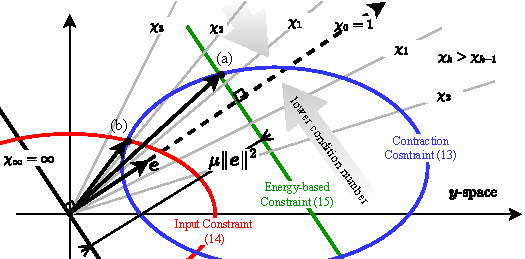
\includegraphics[width=0.75\linewidth]
   {
      figures/scene_first.drawio.pdf
   }
   \caption{
      Illustration of the optimization problem in two-dimensional space.
   }
\label{fig:scene:first}
\end{figure}

For better intuition, in Fig.~\ref{fig:scene:first}, the constraints are illustrated in two-dimensional space.
The minimization of the condition number of $\mm{M}$ is equivalent to minimizing the angle between $\mv{y}$ and $\mv{e}$ as depicted in Fig.~\ref{fig:scene:first}. 
The contraction constraint \eqref{eq:cstr:ctrc:proj} and the input saturation constraint $\mysat(\mv{y})\le0$ restrict the feasible space of $\mv{y}$ in the outside of blue eclipse and the inside of red eclipse, respectively.


The green lines represent the energy-based constraint \eqref{eq:cstr:energy}.


\section{Numerical Validation}

\subsection{Numerical Validation Set Up}

We employed the Lorenz system \MSRY{REF} to validate the proposed method which is represented as follows:
\begin{equation}
   \ddtt
   \underbrace{
      \begin{pmatrix}
         x\\y\\z
      \end{pmatrix}
   }_{=:\mv{\xi}}
   =
   \underbrace{
      \begin{pmatrix}
         \sigma(y-x)
         \\
         x(\rho-z)-y
         \\
         xy-\beta z
      \end{pmatrix}
   }_{=:\mv{f}(\mv{\xi})}
   +
   \underbrace{
      \begin{pmatrix}
         u_x\\u_y\\u_z
      \end{pmatrix}
   }_{=:\mv{u}}
   +
   \underbrace{
      \begin{pmatrix}
         d_x\\d_y\\d_z
      \end{pmatrix}
   }_{=:\mv{d}}
   ,
\end{equation}
where $\sigma=10$, $\rho=28$, and $\beta=\tfrac{8}{3}$ are system parameters.



\subsection{Numerical Validation Results}

\begin{table}[t]
   \renewcommand{\arraystretch}{1.3}
   \caption{Controllers for comparative study.}
   \centering
   % \begin{tabular}{c m{13.5em}}
   \begin{tabular}{c l}
   \hline
   & \textbf{Description} \\
   \hline
   \hline 
   (C$_1$) \protect\colorLine{blue}{solid} & Proposed controller \\ 
   \hline
   (C$_2$) \protect\colorLine{my_cyan}{solid} & CV-STEM (\cite{Tsukamoto:2021ae}) \\
   \hline
   (C$_3$) \protect\colorLine{gray}{solid} & Desired controller, \ie $\mv{u}=\mv{u}_d$ \\
   \hline
   \end{tabular}
   \label{table:controllers}
\end{table}

\begin{figure}[t]
   \centering
   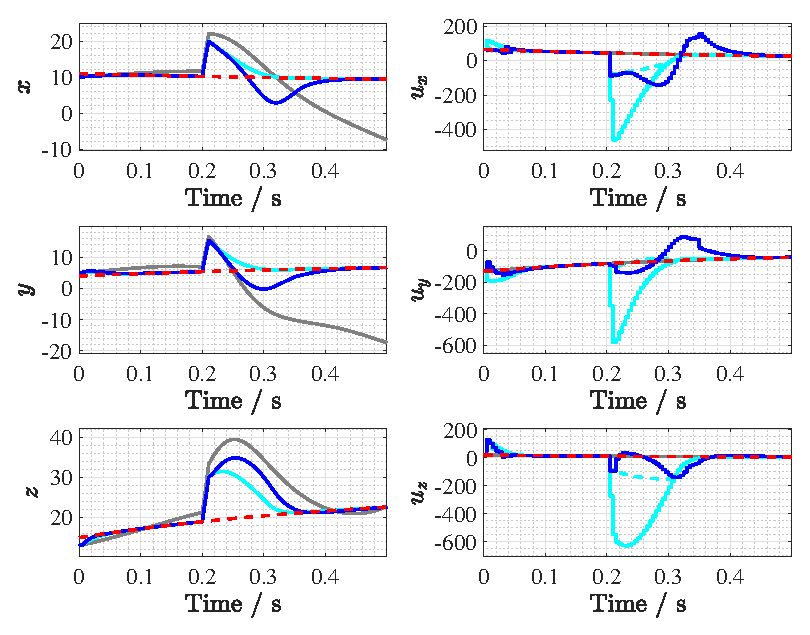
\includegraphics[width=0.99\linewidth]
   {
      src/script_simulation/figures/compare/Fig1.eps
   }
   \caption{
      Numerical validation results of (C$_1$) \protect\colorLine{blue}{solid}, (C$_2$) \protect\colorLine{my_cyan}{solid}, (C$_3$) \protect\colorLine{gray}{solid}, and desired trajectory $x_d$ \protect\colorLine{red}{dashed}   
   }
   \label{fig:sim:result:control}
\end{figure}

\begin{figure}[t]
   \centering
   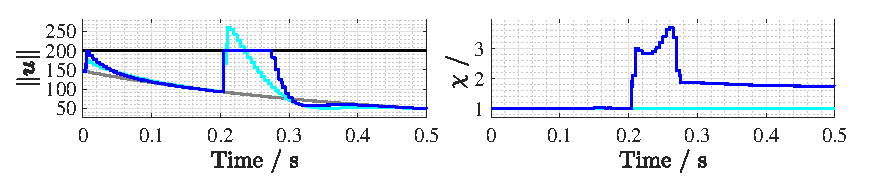
\includegraphics[width=0.99\linewidth]
   {
      src/script_simulation/figures/compare/Fig2.eps
   }
   \caption{
      Optimization results of (C$_1$) \protect\colorLine{blue}{solid} and (C$_2$) \protect\colorLine{my_cyan}{solid}.
   }
   \label{fig:sim:result:opt}
\end{figure}



\section{Conclusion}

In this study, ...

\begin{comment}

\section{Introduction}
This document is a template for \LaTeXe. If you are reading a paper or
PDF version of this document, please download the electronic file
\texttt{ifacconf.tex}. You will also need the class file
\texttt{ifacconf.cls}. Both files are available on the IFAC web site.

Please stick to the format defined by the \texttt{ifacconf} class, and
do not change the margins or the general layout of the paper. It
is especially important that you do not put any running header/footer
or page number in the submitted paper.\footnote{
This is the default for the provided class file.}
Use \emph{italics} for emphasis; do not underline.

Page limits may vary from conference to conference. Please observe the 
page limits of the event for which your paper is intended.

% $\vec$

\section{Procedure for Paper Submission}

Next we see a few subsections.

\subsection{Review Stage}

For submission guidelines, follow instructions on paper submission
system as well as the event website.

Note that conferences impose strict page limits, so it will be better
for you to prepare your initial submission in the camera ready layout
so that you will have a good estimate for the paper
length. Additionally, the effort required for final submission will be
minimal.

\subsection{Equations}

Some words might be appropriate describing equation~(\ref{eq:sample}), if 
we had but time and space enough. 

\begin{equation} \label{eq:sample}
{{\partial F}\over {\partial t}} = D{{\partial^2 F}\over {\partial x^2}}.
\end{equation}

See \cite{Abl:56}, \cite{AbTaRu:54}, \cite{Keo:58} and \cite{Pow:85}.

\subsubsection{Example.} This equation goes far beyond the
celebrated theorem ascribed to the great Pythagoras by his followers.

\begin{thm}   % use the thm environment for theorems
The square of the length of the hypotenuse of a right triangle equals
the sum of the squares of the lengths of the other two sides.
\end{thm}

\begin{pf}    % and the pf environment for proofs
The square of the length of the hypotenuse of a right triangle equals the sum of the squares 
of the lengths of the other two sides.
\end{pf}

%% There are a number of predefined theorem-like environments in
%% ifacconf.cls:
%%
%% \begin{thm} ... \end{thm}            % Theorem
%% \begin{lem} ... \end{lem}            % Lemma
%% \begin{claim} ... \end{claim}        % Claim
%% \begin{conj} ... \end{conj}          % Conjecture
%% \begin{cor} ... \end{cor}            % Corollary
%% \begin{fact} ... \end{fact}          % Fact
%% \begin{hypo} ... \end{hypo}          % Hypothesis
%% \begin{prop} ... \end{prop}          % Proposition
%% \begin{crit} ... \end{crit}          % Criterion

Of course LaTeX manages equations through built-in macros. You may
wish to use the \texttt{amstex} package for enhanced math
capabilities.

\subsection{Figures}

To insert figures, use the \texttt{graphicx} package. Although other
graphics packages can also be used, \texttt{graphicx} is simpler to
use. See  Fig.~\ref{fig:bifurcation} for an example.

\begin{figure}
\begin{center}
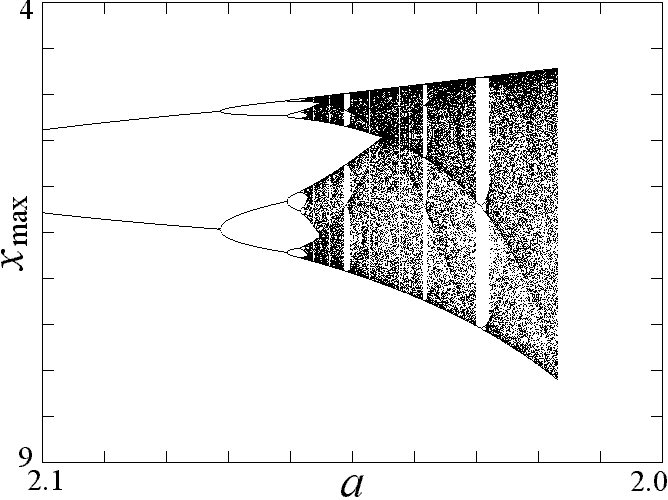
\includegraphics[width=8.4cm]{bifurcation}    % The printed column width is 8.4 cm.
\caption{Bifurcation: Plot of local maxima of $x$ with damping $a$ decreasing} 
\label{fig:bifurcation}
\end{center}
\end{figure}

Figures must be centered, and have a caption at the bottom. 

\subsection{Tables}
Tables must be centered and have a caption above them, numbered with
Arabic numerals. See table~\ref{tb:margins} for an example.

\begin{table}[hb]
\begin{center}
\caption{Margin settings}\label{tb:margins}
\begin{tabular}{cccc}
Page & Top & Bottom & Left/Right \\\hline
First & 3.5 & 2.5 & 1.5 \\
Rest & 2.5 & 2.5 & 1.5 \\ \hline
\end{tabular}
\end{center}
\end{table}

\subsection{Final Stage}

Authors are expected to mind the margins diligently.  Papers need to
be stamped with event data and paginated for inclusion in the
proceedings. If your manuscript bleeds into margins, you will be
required to resubmit and delay the proceedings preparation in the
process.

\subsubsection{Page margins.} See table~\ref{tb:margins} for the
page margins specification. All dimensions are in \emph{centimeters}.


\subsection{PDF Creation}

All fonts must be embedded/subsetted in the PDF file. Use one of the
following tools to produce a good quality PDF file:

\subsubsection{PDFLaTeX} is a special version of LaTeX by Han The
Thanh which produces PDF output directly using Type-1 fonts instead of
the standard \texttt{dvi} file. It accepts figures in JPEG, PNG, and PDF
formats, but not PostScript. Encapsulated PostScript figures can be
converted to PDF with the \texttt{epstopdf} tool or with Adobe Acrobat
Distiller.

\subsubsection{Generating PDF from PostScript} is the classical way of
producing PDF files from LaTeX. The steps are:

\begin{enumerate}
  \item Produce a \texttt{dvi} file by running \texttt{latex} twice.
  \item Produce a PostScript (\texttt{ps}) file with \texttt{dvips}.
  \item Produce a PDF file with \texttt{ps2pdf} or Adobe Acrobat
  Distiller.
\end{enumerate}

\subsection{Copyright Form}

IFAC will put in place an electronic copyright transfer system in due
course. Please \emph{do not} send copyright forms by mail or fax. More
information on this will be made available on IFAC website.


\section{Units}

Use SI as primary units. Other units may be used as secondary units
(in parentheses). This applies to papers in data storage. For example,
write ``$15\,\mathrm{Gb}/\mathrm{cm}^2$ ($100\,\mathrm{Gb}/\mathrm{in}^2$)''. 
An exception is when
English units are used as identifiers in trade, such as ``3.5 in
disk drive''. Avoid combining SI and other units, such as current in
amperes and magnetic field in oersteds. This often leads to confusion
because equations do not balance dimensionally. If you must use mixed
units, clearly state the units for each quantity in an equation.  The
SI unit for magnetic field strength $\mathbf{H}$ is $\mathrm{A}/\mathrm{m}$. However, if you wish to
use units of $\mathrm{T}$, either refer to magnetic flux density $\mathbf{B}$ or
magnetic field strength symbolized as $\mu_0\,\mathbf{H}$. Use the center dot to
separate compound units, e.g., ``$\mathrm{A} \cdot \mathrm{m}^2$''.

\section{Helpful Hints}

\subsection{Figures and Tables}

Figure axis labels are often a source of confusion. Use words rather
than symbols. As an example, write the quantity ``Magnetization'', or
``Magnetization M'', not just ``M''. Put units in parentheses. Do not
label axes only with units.  For example, write ``Magnetization
($\mathrm{A}/\mathrm{m}$)'' or ``Magnetization ($\mathrm{A} \mathrm{m}^{-1}$)'', not just
 ``$\mathrm{A}/\mathrm{m}$''. Do not
label axes with a ratio of quantities and units. For example, write
``Temperature ($\mathrm{K}$)'', not ``$\mbox{Temperature}/\mathrm{K}$''.

Multipliers can be especially confusing. Write ``Magnetization
($\mathrm{kA}/\mathrm{m}$)'' or ``Magnetization ($10^3 \mathrm{A}/\mathrm{m}$)''. Do not write
``Magnetization $(\mathrm{A}/\mathrm{m}) \times 1000$'' because the reader would not know
whether the axis label means $16000\,\mathrm{A}/\mathrm{m}$ or $0.016\,\mathrm{A}/\mathrm{m}$.

\subsection{References}

Use Harvard style references (see at the end of this document). With
\LaTeX, you can process an external bibliography database 
using \texttt{bibtex},\footnote{In this case you will also need the \texttt{ifacconf.bst}
file, which is part of the \texttt{ifaconf} package.}
or insert it directly into the reference section. Footnotes should be avoided as
far as possible.  Please note that the references at the end of this
document are in the preferred referencing style. Papers that have not
been published should be cited as ``unpublished''.  Capitalize only the
first word in a paper title, except for proper nouns and element
symbols.

\subsection{Abbreviations and Acronyms}

Define abbreviations and acronyms the first time they are used in the
text, even after they have already been defined in the
abstract. Abbreviations such as IFAC, SI, ac, and dc do not have to be
defined. Abbreviations that incorporate periods should not have
spaces: write ``C.N.R.S.'', not ``C. N. R. S.'' Do not use abbreviations
in the title unless they are unavoidable (for example, ``IFAC'' in the
title of this article).

\subsection{Equations}

Number equations consecutively with equation numbers in parentheses
flush with the right margin, as in (\ref{eq:sample}).  To make your equations more
compact, you may use the solidus ($/$), the $\exp$ function, or
appropriate exponents. Use parentheses to avoid ambiguities in
denominators. Punctuate equations when they are part of a sentence, as
in

\begin{equation} \label{eq:sample2}
\begin{array}{ll}
\int_0^{r_2} & F (r, \varphi ) dr d\varphi = [\sigma r_2 / (2 \mu_0 )] \\
& \cdot \int_0^{\inf} exp(-\lambda |z_j - z_i |) \lambda^{-1} J_1 (\lambda  r_2 ) J_0 (\lambda r_i ) d\lambda 
\end{array}
\end{equation}

Be sure that the symbols in your equation have been defined before the
equation appears or immediately following. Italicize symbols ($T$
might refer to temperature, but T is the unit tesla). Refer to
``(\ref{eq:sample})'', not ``Eq. (\ref{eq:sample})'' or ``equation
(\ref{eq:sample})'', except at the beginning of a sentence: ``Equation
(\ref{eq:sample}) is \ldots''.

\subsection{Other Recommendations}

Use one space after periods and colons. Hyphenate complex modifiers:
``zero-field-cooled magnetization''. Avoid dangling participles, such
as, ``Using (1), the potential was calculated'' (it is not clear who or
what used (1)). Write instead: ``The potential was calculated by using
(1)'', or ``Using (1), we calculated the potential''.

A parenthetical statement at the end of a sentence is punctuated
outside of the closing parenthesis (like this). (A parenthetical
sentence is punctuated within the parentheses.) Avoid contractions;
for example, write ``do not'' instead of ``don' t''. The serial comma
is preferred: ``A, B, and C'' instead of ``A, B and C''.


\section{Conclusion}

A conclusion section is not required. Although a conclusion may review
the main points of the paper, do not replicate the abstract as the
conclusion. A conclusion might elaborate on the importance of the work
or suggest applications and extensions.

\end{comment}

\begin{ack}
Place acknowledgments here.
\end{ack}

\bibliography{template/refs, localRefs}             % bib file to produce the bibliography
                                    % with bibtex (preferred)

% \appendix
% \section{SDC Derivation} \label{sec:appendix:SDC}

% In this appendix, the SDC $\mathbb{A}$ will be derived in detail.
% First, we follow the definition of the SDC in \eqref{eq:SDC} as follows:
% \begin{equation}
%    \begin{aligned}
%       \mathbb{A}
%       =&
%       \textstyle\int_0^1 
%       \left[
%          \pptfrac{}{\mv{x}}
%          \left(
%             \mm{A} \mv{x}
%             +
%             \mm{B} \mv{u}_d
%          \right)
%       \right]
%       \big(
%          c \mv{x} + (1-c) \mv{x}_d
%       \big)
%       \,
%       \der c
%       \\
%       =&
%       \textstyle\int_0^1
%       \left[
%          \left(
%             \mm{A}
%             +
%             \begin{bmatrix}
%                0 & 0 
%                \\
%                b_1 & 0
%             \end{bmatrix}
%          \right)
%       \right]
%       \big(
%          c \mv{x} + (1-c) \mv{x}_d      
%       \big)
%       \,
%       \der c
%       ,
%    \end{aligned}
% \end{equation}
% where 
% $
%    b_1
%    :=
%    b_1(\mv{x},\mv{x}_d)
%    = 
%    - \tfrac{3P^2\Phi}{2J}
%    \left(
%       \cos(P x_1) {u_1}_d
%       +
%       \sin(P x_1) {u_2}_d
%    \right)
% $.
% Then, we can rewrite the SDC as follows:
% \begin{equation} \label{eq:SDC:explicit:2}
%    \mathbb{A}
%    =
%    \begin{bmatrix}
%       0 & 1 \\
%       b_2(\mv{x},\mv{x}_d) & -\tfrac{f_v}{J}
%    \end{bmatrix}
%    ,
% \end{equation}
% where 
% \begin{equation*}
%    \begin{aligned}
%       b_2(\mv{x},\mv{x}_d)
%       :=&
%       \tfrac{3P\Phi}{2J(x_1-{x_1}_d)}
%       \big[
%          \left\{
%             \sin(P x_1)
%             -
%             \sin(P{ x_1}_d)
%          \right\}
%          {u_1}_d
%       \\
%       &
%          +
%          \left\{
%             \cos(P x_1)
%             -
%             \cos(P {x_1}_d)
%          \right\}
%          {u_2}_d
%       \big]
%       .
%    \end{aligned}
% \end{equation*}

\end{document}
